%----------------------------------------------------------------------------------------
%	PACKAGES AND THEMES
%----------------------------------------------------------------------------------------

\documentclass{beamer}
\usepackage[]{algorithm2e}
\mode<presentation> {

\usetheme{default}
%\usetheme{Dresden}
%\usetheme{Malmoe}
%\usetheme{Singapore}

\setbeamertemplate{footline}
}

\usepackage{graphicx} % Allows including images
\usepackage{booktabs} % Allows the use of \toprule, \midrule and \bottomrule in tables

%----------------------------------------------------------------------------------------
%	TITLE PAGE
%----------------------------------------------------------------------------------------

\title[Protein Docking]{Protein Docking}

\author{Peter M\"uhlbacher}

\date{\today}

\begin{document}

\begin{frame}
\titlepage
\end{frame}

%----------------------------------------------------------------------------------------
%	PRESENTATION SLIDES
%----------------------------------------------------------------------------------------

\begin{frame}
\frametitle{What Are Amino Acids?}

\begin{figure}
\caption{Illustration of an amino acid. \cite{neumaier}}
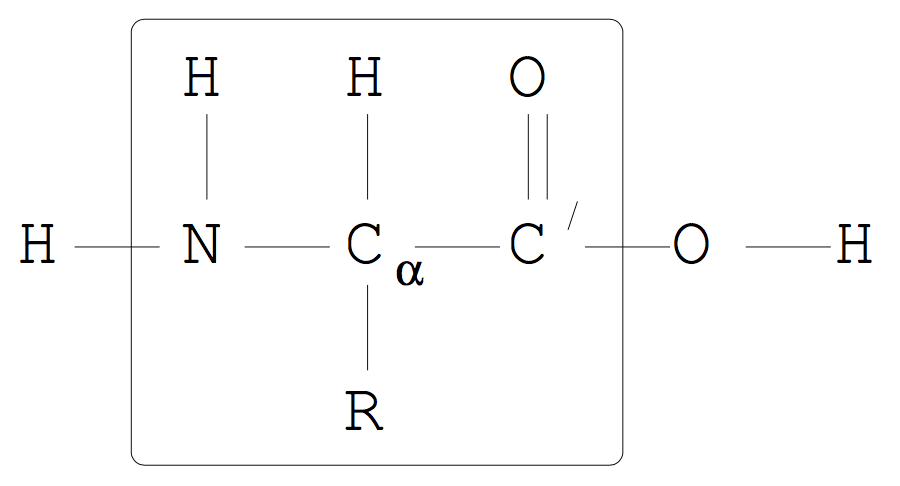
\includegraphics[width=0.7\linewidth]{aminoacid.png}
\end{figure}

\begin{itemize}
	\item amino acids polymerize in a specific sequence to a chain
	\item the repeating $N,C_\alpha,C$-pattern is called the protein's backbone
\end{itemize}

\end{frame}

%------------------------------------------------

\begin{frame}
\frametitle{Structures}

\begin{block}{Primary Structure}
amino acid sequence
\end{block}

\begin{block}{Secondary Structure}
spatial arrangement of amino acid residues that are nearby in the sequence
\end{block}

\begin{block}{Tertiary Structure}
its three-dimensional structure, as defined by the atomic coordinates
\end{block}

\begin{block}{Quaternary Structure}
spatial arrangement of multiple folded proteins and the nature of their interactions \cite{berg}
\end{block}


\end{frame}

%------------------------------------------------

\begin{frame}
\frametitle{What Is Protein Docking And Why Is It Important?}
\begin{block}{The Problem}
\begin{itemize}
	\item given tertiary structures, find the most likely quaternary structure
	\item evaluate its affinity
\end{itemize}
\end{block}

\begin{block}{Examples For Quaternary Structures}
\begin{itemize}
	\item hemoglobin
	\item DNA polymerase
	\item ion channels
\end{itemize}
Understanding how proteins interact $\rightarrow$ drug design
\end{block}
\end{frame}

%------------------------------------------------

\begin{frame}
\frametitle{Vocabulary}

\begin{columns}
\column{.45\textwidth}
\begin{itemize}[<+->]
	\item bond angle
	\item dihedral angle
	\item internal coordinates
	\item absolute coordinates
\end{itemize}
\column{.5\textwidth}
\only<1-2>{
\begin{figure}
\only<1-1>{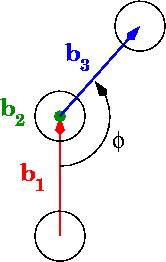
\includegraphics[width=.7\linewidth]{bondangle.png}}
\only<2-2>{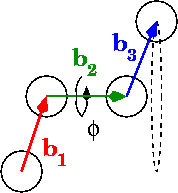
\includegraphics[width=.8\linewidth]{dihedralangle.png}}
\end{figure}
}\only<3-3>{set of bond lenghts, bond angles and dihedral angles; usually only some dihedral angles are allowed to vary though; protein can be seen as a tree-like graph structure\\~\\useful to alter a molecule in a chemically meaningful way}\only<4-4>{set of cartesian coordinates of every single atom in a molecule\\~\\useful to calculate potentials}
\end{columns}

\end{frame}

%------------------------------------------------

\begin{frame}
\frametitle{Different Approaches}
The problem can be casted as a minimization problem: $\text{argmin}_{X} U(X)$. One can differentiate between several approaches.
\begin{block}{Classes of Potential Functions}
\begin{itemize}
	\item \textbf{Force fields:} Typically, the potential $U$ is a sum over bond, angle, dihedral angle, electrostatic and van der Waals energies.
	\item \textbf{Knowledge-based/empirical methods:} Compare segments with experimentally determined data.
\end{itemize}
\end{block}

\begin{block}{Choosing a Set of Parameters}
\begin{itemize}
	\item \textbf{Rigid docking:} The parameters $X$ consist of translation and rotation of the smaller protein in $\mathbb R^3$.
	\item \textbf{Flexible docking:} In addition to the 6 parameters of rigid docking, internal parameters (mostly dihedral angles, as bond angles and lengths are relatively stable) are used.
\end{itemize}
\end{block}

\end{frame}

%------------------------------------------------

\begin{frame}
\frametitle{The Potential Function In Use}
\begin{itemize}
	\item let $X = x,y,z,\alpha,\beta,\gamma,\theta_1,\dots,\theta_n$ free parameters,
	\item $M^1(X)=M^1$ be the flexible and $M^2$ the fixed molecule,
	\item $LJ_{M_i,M_j}$ the Lennard-Jones potential, modelling pairwise van der Waals forces, depending on the types of the atoms $M_i,M_j$ and
	\item $\|M_i-M_j\|$ the euclidian distance of their cartesian coordinates.
\end{itemize}

$$U(X) =
\underbrace{\sum_{i=1}^{|M^1|}\sum_{j>i}^{|M^1|}LJ_{M^1_i,M^1_j}(\|M^1_i-M^1_j\|)}_{\text{internal energy of }M^1} + \underbrace{\sum_{i=1}^{|M^1|}\sum_{j=1}^{|M^2|}LJ_{M^1_i,M^2_j}(\|M^1_i-M^2_j\|)}_{\text{interaction of }M^1\text{ and }M^2}$$

\end{frame}

%------------------------------------------------

\begin{frame}
\frametitle{Physical Interpretation of $LJ$}
Setting $$LJ_{M_i,M_j}(r) = \frac{A_{M_i,M_j}}{r^{12}}-\frac{B_{M_i,M_j}}{r^6}$$ for $A_{M_i,M_j},B_{M_i,M_j}\in\mathbb R^+$ \only<1-1>{yields the following with a strong divergence at $r=0$.
\begin{figure}
%\caption{Illustration of an amino acid.}
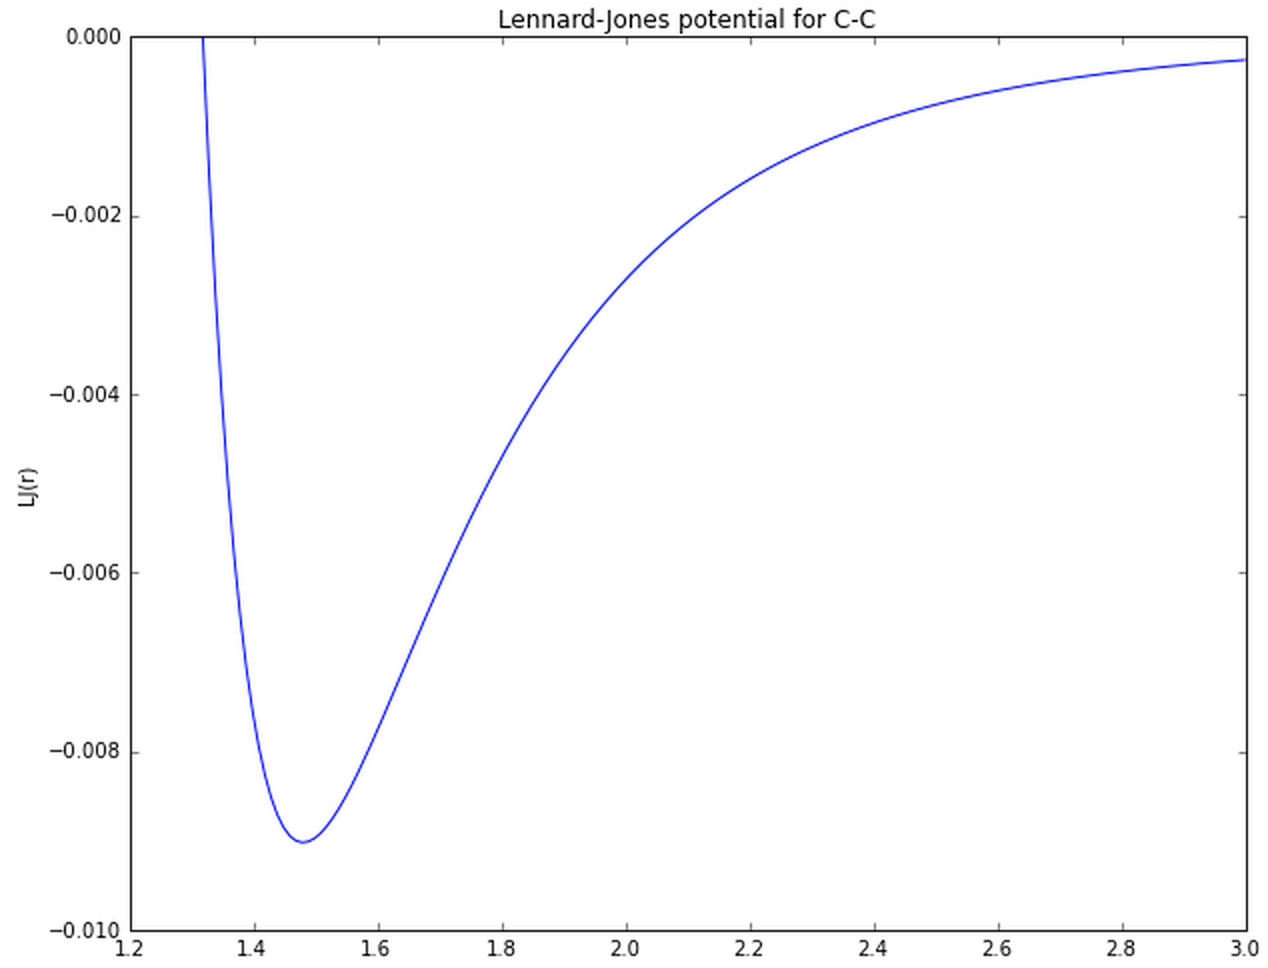
\includegraphics[width=0.6\linewidth]{LJ.png}
\end{figure}
}\only<2->{
leads to the following interpretation:
\begin{itemize}
	\item $A$ corresponds to the strength of the Pauli-repulsion.
	\item $B$ corresponds to the attractive long-range term.
	\item $\varepsilon := \underset{r}{\operatorname{min}}LJ(r) = \frac{B^2}{4A}$ is the depth of the potential well. 
	\item $r_m := \underset{r}{\operatorname{argmin}}LJ(r) = \sqrt[6]{2\frac{A}{B}}$ determines the equilibrium distance of the two elements $M_i,M_j$.
\end{itemize}
}

\end{frame}

%------------------------------------------------

\begin{frame}
\frametitle{Meaningfulness of the Potential Function}
\begin{columns}[t]

\column{.45\textwidth}
\textbf{cons}
\begin{itemize}
	\item Various other physical properties are neglected, e.g. dipole-dipole interactions leading to secondary structures like the $\alpha$-helix.
\end{itemize}

\column{.5\textwidth}
\textbf{\only<3->{``}pros\only<3->{''}}
\begin{itemize}
	\item<2-> Speed.
	\item<3-> All models are simply fitted mathematical functions $\rightarrow$ treating $C,C_\alpha,O,N,\dots$ as different elements might account for other physical properties to some extent.
	\item<4-> It works to a certain extent, i.e. $\nabla_X U(X)\approx 0$ if $X$ describes the initial configuration which should be an equilibrium state.
\end{itemize}

\end{columns}


\end{frame}

%------------------------------------------------

\begin{frame}
\frametitle{Finding Optimal Parameters}
Observe that ``$M$ is in equilibrium'' $\Leftrightarrow \nabla_X U_{A,B}(X_M,M)=0$.
Thus, it is natural to choose $A,B \in\mathbb (R^+)^{n\times n}$, where $n$ is the number of different substances one wants to differentiate between, as

$$\underset{A,B}{\operatorname{argmin}} \sum_{M^i\in\text{training set}}\|\nabla_X U_{A,B}(X_{M^i},M^i)\|.$$

However, this is an overdetermined system $\rightarrow$ fix $A_{11} = \textit{const}$ and express all other parameters in terms of $A_{11}$, i.e.: $\tilde A_{ij} = A_{11}A_{ij}$, $\tilde B_{ij} = A_{11}B_{ij}$.

\end{frame}

%------------------------------------------------

\begin{frame}
\frametitle{Finding Optimal Parameters}

\begin{figure}
\caption{Projection of the optimization problem in $n(n+1)-1$ dimensions onto a $1$-dimensional subspace ($B_{11}$ is the only non-constant parameter, $A_{ij}=1, B_{ij}=B_{11}$)}
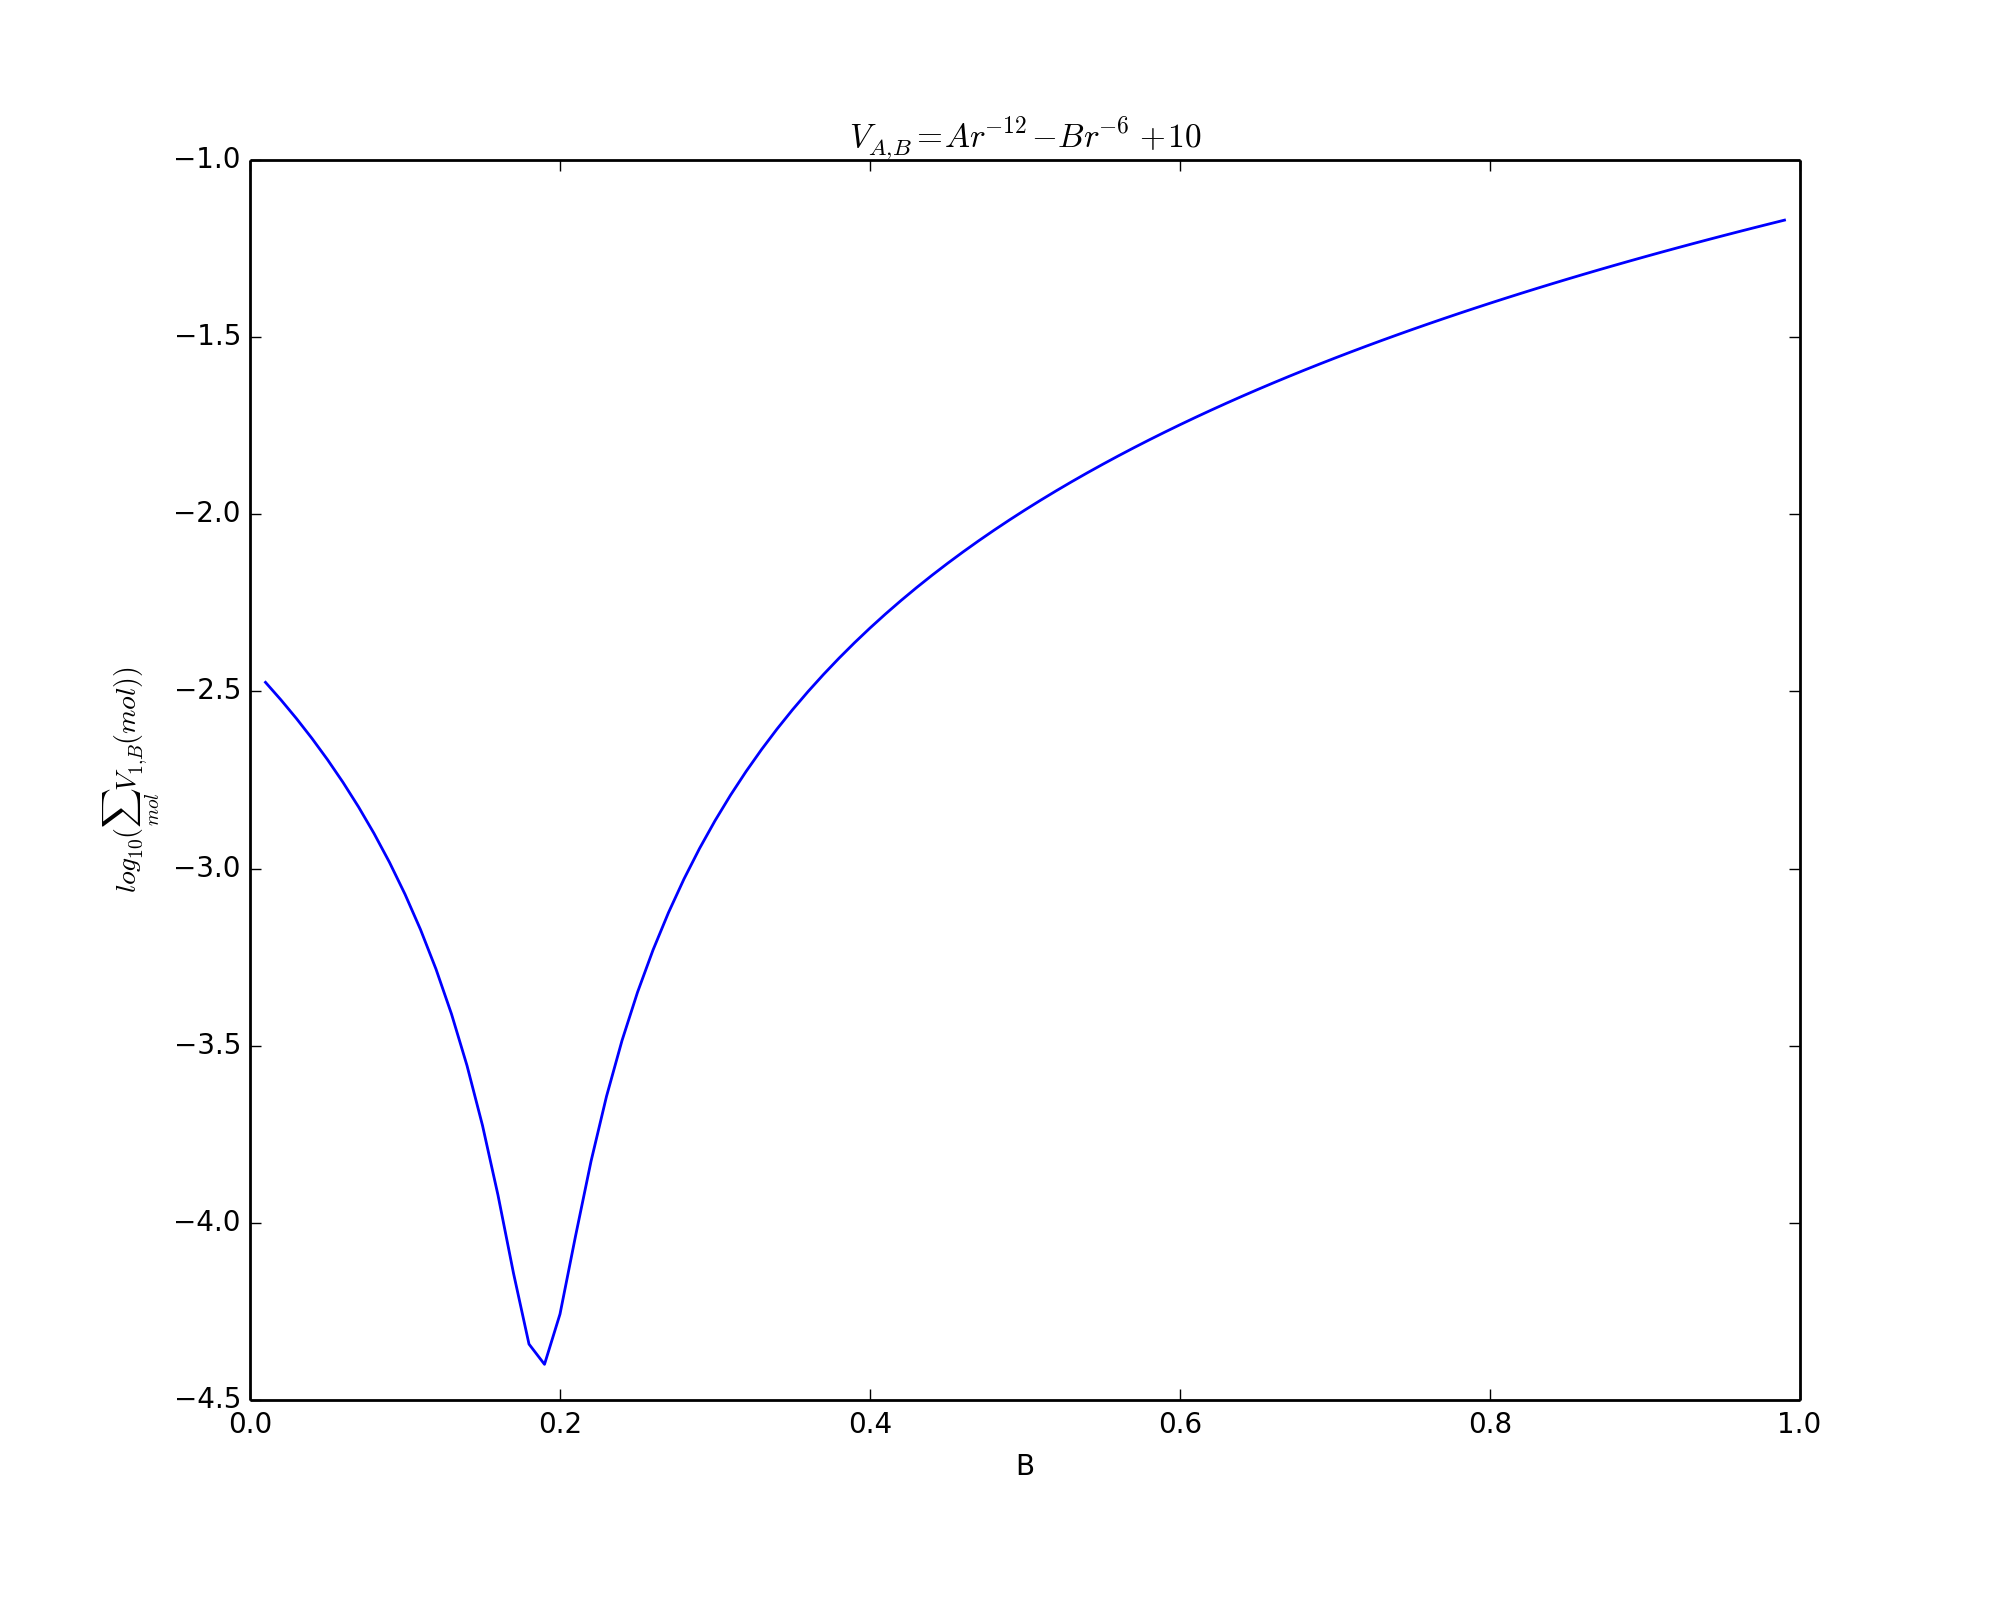
\includegraphics[width=0.75\linewidth]{sumoverU.png}
\end{figure}


\end{frame}

%------------------------------------------------

\begin{frame}
\frametitle{Numerical Challenges}
\begin{block}{Conversion Between Internal And Absolute Coordinates}
While we want to write the potential as a function of the internal coordinates, it can only be calculated in terms of absolute coordinates $\rightarrow$ conversion is done often and should thus be implemented efficiently, i.e. minimize rounding errors and duration of computation
\end{block}

\begin{block}{Computation of the Gradient}
The potential is not simply a sum over rational functions as the distance between two atoms depends on the internal coordinates $\rightarrow$ the above conversion has to be included as well; as a result, computing the gradient explicitly is not only a tedious, but also an unnecessary task because of accumulating rounding errors $\rightarrow$ automatic backwards differentiation
\end{block}
\end{frame}

%------------------------------------------------

\begin{frame}
\Huge{\centerline{The End}}
\end{frame}

%------------------------------------------------

\begin{frame}
\frametitle{References}
\footnotesize{
\begin{thebibliography}{99} % Beamer does not support BibTeX so references must be inserted manually as below
\bibitem[Neumaier, 2006]{neumaier} Arnold Neumaier (2006)
\newblock Molecular Modeling of Proteins
\bibitem[Berg, Tymoczko, Stryer, 2002]{berg} Berg JM, Tymoczko JL, Stryer L. (2002)
\newblock Biochemistry. 5th edition.
\end{thebibliography}
}
\end{frame}

%----------------------------------------------------------------------------------------

\end{document}